% !TEX root = ../thesis_main.tex



%%%% --- * --- %%%%	
\chapter[Notation]{Comparing Notation between Holstein and JTW}
\label{appendix_notation}
%%%%%\note[color=tag]{Un-pinken the pink things in Tables~\ref{table:compare_notation_angularmomentum}, \ref{table:compare_notation_multipoles}.  Probably rephrase the descriptions for Tables~\ref{table:compare_notation_kinematic}, \ref{table:compare_notation_multipoles}. }
%\note[color=jb]{JB on how to triage Appendix C:   
%\\
%keep after: 
%\\
%   C.1: keep 1st two sentences, discard next few.
%\\
%   C.2 Remove subsection title, replace by one sentence 'This section includes handwritten notes.' without further apology. We can't pay you anymore
%to make nice Latex. If the committee or Gerald objects to complex handwritten notes, App. C -> internal.}

%%%%%\note{I see some stuff in my old Appendix D that needs to be moved (in here?  Or maybe in Old Appendix E) before it goes away forever.}
%%%%%\note[color=jb]{JB:  Appendix C has some redundancies with B. You will have to sort that out.  (n.b.:  from context, it's less clear which appendices he's actually talking about, but whatever, there's certainly redundancies all around.}

%%%%%%\section{Comparing Notation between Holstein and JTW}
%%%%%\FloatBarrier
%%%%%\section{Relations between Terms within the PDFs}
%%%%%\label{sec:imported_equations}
%%%%%\note[color=tag]{Rephrase the descriptive paragraph in Sec.~\ref{sec:imported_equations}.  Is this content redundant?}
%%%%%Here are some equations.  I want to keep these somewhere in this chapter.  For the equations below, I am intentionally not including the ROC terms.  We take only enough Holstein terms to construct the expressions JTW gives us.
%%%%%%\note{In fact, 
%%%%%%\beq 
%%%%%%\xi = G_v^2 \, \cos\theta_C \, f_1(E)
%%%%%%\eeq  
%%%%%%}
%%%%%

%\section{Comparison Guide}
	This section provides several equations and tables intended to be used as a quick reference for comparing differences in notation, sign convention, and normalization between two different descriptions of the beta decay probability distribution.  This section also includes several pages of handwritten notes.

%	 a short guide to differences in notation, sign convention, and normalization.  There are several tables here, chosen to aid in conversion between the two conventions.  
%In the mean time, here's a bunch of old handwritten notes on the topic, that I'll eventually have to typeset and process into something intelligible.  

The following equations provide a term-by-term comparison between the Holstein and JTW conventions, intentionally neglecting ROC terms.  % i.e., we take only enough Holstein terms to construct the expressions JTW gives us.
\bea
\xi &=& G_v^2 \, \cos\theta_C \, f_1(E) \\
a_{\beta\nu} &=& f_2(E) \: / \: f_1(E) \\
\frac{\langle\vec{J}\rangle}{J} \cdot \frac{\vec{p}}{E} \,\, A_\beta 
  &=& \Lambda_1 \hat{n}\cdot \frac{\vec{p}}{E} \, f_4(E) \:/\: f_1(E) \\
\frac{\langle\vec{J}\rangle}{J} \cdot \frac{\vec{p}_\nu}{E_\nu} B_\nu  
  &=& \Lambda_1 \hat{n} \cdot \vec{k} \;\;\, f_6(E) \:/\: f_1(E) \\
\frac{\langle\vec{J}\rangle}{J} \cdot \frac{\left( \vec{p} \times \vec{p}_\nu \right)}{E_{} E_\nu} D_{\mathrm{TR}} 
  &=& \Lambda_1 \hat{n} \cdot ( \frac{\vec{p}}{E} \times \hat{k} \,) \;\; f_8(E) \:/\: f_1(E)
\end{eqnarray}
\begin{eqnarray}
&& \!\!\!\! \!\!\!\! 
\left[ \frac{J(J+1) - 3\langle (\vec{J}\cdot\hat{j})^2 \rangle}{J(2J-1)} \right] \!\!\!
\left[\frac{1}{3} \frac{\vec{p}\cdot\vec{p}_\nu }{E_{} E_\nu} - \frac{ (\vec{p}\cdot\hat{j}) (\vec{p}_\nu \cdot\hat{j} ) }{E_{} E_\nu} \right]c_{\mathrm{align}}
\nonumber\\
&& \;\;\;\; \;\;=\;\; \Lambda_2 \! \left[(\hat{n}\cdot\frac{\vec{p}}{E})(\hat{n}\cdot\hat{k})  - \frac{1}{3} (\frac{\vec{p}}{E}\cdot\hat{k} \,)\right] \; f_{12}(E) \:/\: f_1(E)
\end{eqnarray}


%Here's a table.
% !TEX root = ../thesis_main.tex
%
%
%
%%%% --- * --- %%%%	
\renewcommand{\arraystretch}{1.6}
\begin{table}[h!!!!t]
	\begin{center}
	\begin{tabular}{ | l | l | p{3.35in} | }
		\multicolumn{1}{c}{Holstein} 				& \multicolumn{1}{c}{JTW} 					& \multicolumn{1}{c}{Comments}
		\\  \hline
		$\hatn$ 									& $\hatj$									& Nuclear polarization unit vector.  Also the axis of quantization.  %In Holstein, this is actually just the axis of quantization, and the mathematical framework is provided such that it need not be aligned with the polarization.  However, JTW makes the simplification that the axis of quantization and the axis of polarization are the same, so we will do the likewise here.  \comment{(is this even true?)}
		\\  \hline
		$\hatk$ 									& $\frac{\vecpnu}{E_\nu}$					& Neutrino emission direction unit vector.  Neutrinos are always treated as massless.
		\\  \hline
		$\bm{\vec{p}} $								& $\bm{\vec{p}_e}$							& Beta momentum.  We use $\bm{\vec{p}_\beta}$ in this document.
		\\  \hline
		$E$											& $E_e$										& Beta energy.  We use $\Ebeta$ here.
		\\  \hline
		$q$											& $E_\nu$									& Neutrino energy.  Because JTW does not include ROC, their treatment uses $E_\nu$ only to aid clarity, rather than as an independent variable.  Holstein claims that $q$ is a four-vector, but that cannot be strictly true since $q^2 \neq - m_\nu c^2$.
		\\  \hline
	\end{tabular}
	\end{center}
	\caption[Notation Guide]{A comparison of some kinematic terms in JTW~\cite{jtw}~\cite{jtw_coulomb} and Holstein~\cite{holstein}.}
	\label{table:compare_notation}
\end{table}
\renewcommand{\arraystretch}{1}
%
%        % table:compare_notation_kinematic

%Here's another table.
% !TEX root = ../thesis_main.tex
%
%
%
%%%% --- * --- %%%%	
\renewcommand{\arraystretch}{1.6}
\begin{table}[h!!!!t]
	\begin{center}
	\begin{tabular}{ | l | l | p{3.35in} | }
		\multicolumn{1}{c}{Holstein} 			& \multicolumn{1}{c}{JTW} 		& \multicolumn{1}{c}{Comments}
		\\  \hline
		$u$ 									& $J$							& Initial state total nuclear angular momentum.
		\\  \hline
		$v$ 									& $J^\prime$					& Final state total nuclear angular momentum.
		\\  \hline
		$s$										& No equivalent?				& \comment{Umm...  I should check on this.}
		\\  \hline
	\end{tabular}
	\end{center}
	\caption[Angular Momentum Notation]{A comparison of some angular momenta in JTW~\cite{jtw}~\cite{jtw_coulomb} and Holstein~\cite{holstein}.}
	\label{table:compare_notation_angularmomentum}
\end{table}
\renewcommand{\arraystretch}{1}
%
%  % table:compare_notation_angularmomentum

%Here's a third table.
% !TEX root = ../thesis_main.tex
%
%
%
%%%% --- * --- %%%%	
\renewcommand{\arraystretch}{1.6}
\begin{table}[h!!!!t]
	\begin{center}
	\begin{tabular}{ | l | l | l | p{2.35in} | }
		\multicolumn{1}{c}{Holstein} 				& \multicolumn{1}{c}{JTW} 					& \multicolumn{1}{c}{Thesis} 				& \multicolumn{1}{c}{Comments}
		\\  \hline
		$G_v^2 \, \cos\theta_C \, f_1(E)$  			& $\xi$    									& $\xi(\Ebeta)$  							& Normalization.  Proportional to the fractional decay rate.
		\\  \hline
		$\hat{n}$ 									& $\mathbf{j}$								& $\hatj$									& Nuclear polarization unit vector.  Also the axis of quantization.  %In Holstein, this is actually just the axis of quantization, and the mathematical framework is provided such that it need not be aligned with the polarization.  However, JTW makes the simplification that the axis of quantization and the axis of polarization are the same, so we will do the likewise here.  \comment{(is this even true?)}
		\\  \hline
		$J$											& $J$ 										& 											& Total nuclear angular momentum quantum number
		\\  \hline
		$\langle M \rangle$							& $ \left| \langle \mathbf{J} \rangle \right| $ 			& 											& Angular momentum projection along the axis of quantization
		\\  \hline
		$\Lambda^{(1)}\hat{n} = \frac{\langle M \rangle}{J} \hat{n} $		& $\frac{\langle \mathbf{J} \rangle}{J}$ 	& $\Lambda_{1}\hatn $ 						& Dipole element vector.  Proportional to nuclear polarization. 
		\\  \hline
%%%%%%		$\Lambda^{(1)} = \frac{\langle M \rangle}{J} $		& ...								& $\Lambda_{1} $ 							& ...
%%%%%%		\\  \hline 
%		\\[6pt]  \hline \rule{0pt}{18pt}
		$\Lambda^{(2)}$ 							& $\TalignExpand \frac{(2J-1)}{(J+1)}$ 		& $\Talign(\vecJ) \frac{(2J-1)}{(J+1)}$ 	& Quadrupole element
		\\  \hline 
		$\Lambda^{(3)}$								& No equivalent								& $\Lambda_{3} $							& Octopole element
		\\  \hline
		$\Lambda^{(4)}$								& No equivalent								& $\Lambda_{4} $							& Hexadecapole element
%		\\  \hline
%		$\hatn$ 									& $\hatj$									& & Nuclear polarization unit vector.
%		\\  \hline
%		$\hatk$ 									& $\frac{\vecpnu}{E_\nu}$					& & Neutrino emission direction unit vector.  Neutrinos are always treated as massless.
%		\\  \hline
%		$\bm{\vec{p}} $								& $\bm{\vec{p}_e}$							& & Beta momentum.  We use $\bm{\vec{p}_\beta}$ in this document.
		\\  \hline
	\end{tabular}
	\end{center}
%%%%%%	\note{Fix the ``...'' !}
	\caption[Multipole Notation]{A comparison of terms relating to multipole elements and their normalizations in JTW~\cite{jtw}~\cite{jtw_coulomb} and Holstein~\cite{holstein}~\cite{holstein_errata}.}
	\label{table:compare_notation_multipoles}
\end{table}
\renewcommand{\arraystretch}{1}
%
%
%
%\renewcommand{\arraystretch}{1.6}
%\begin{table}[h!!!!t]
%	\begin{center}
%	\begin{tabular}{ | l | l | p{3.35in} | }
%		\multicolumn{1}{c}{JTW} 				& \multicolumn{1}{c}{Holstein} 				& \multicolumn{1}{c}{Comments}
%		\\  \hline
%		$\xi$    								& $G_v^2 \, \cos\theta_C \, f_1(E_\beta)$  	& Normalization.  Proportional to the decay rate.
%		\\  \hline
%		$\hatj$									& $\hatn$ 									& Nuclear polarization unit vector.
%		\\  \hline
%		$\frac{\vecJ}{J}$ 						& $\Lambda_1\hatn $							& Dipole element vector.  Proportional to nuclear polarization.
%%		\\[6pt]  \hline &\\[-6pt]
%		\\  \hline 
%%		\\[6pt]  \hline \rule{0pt}{18pt}
%		$\Talign(\vecJ) \frac{(2J-1)}{(J+1)}$ 	& $\Lambda_2$ 								& Quadrupole element.
%		\\  \hline 
%		No equivalent							& $\Lambda_3$								& Octopole element.
%		\\  \hline
%	\end{tabular}
%	\end{center}
%	\caption[Notation Guide]{A table comparing equivalent terms in Holstein and JTW.}
%	\label{table:compare_notation}
%\end{table}
%
%\renewcommand{\arraystretch}{1}       % table:compare_notation_multipoles
%
%Here's a fourth table.
% !TEX root = ../thesis_main.tex
%
%
%
%%%% --- * --- %%%%	
\renewcommand{\arraystretch}{1.7}
\begin{table}[h!!!!t]
\vspace*{-2cm}                     % KLUDGE
	\begin{center}
	\begin{tabular}{ | l  c  r  c  l | }
		\multicolumn{1}{c}{Term} &  & \multicolumn{3}{c}{Integral} 					
		\\  \hline
		$\displaystyle f_1(\Ebeta)$	& $  \;\;\;\;\;\;\; \leftrightarrow  \;\;\;\;\;\;\; $ & $\displaystyle \int 1 \, \dOmegakhat$ 	& $\displaystyle=$ & $\displaystyle 4\pi$ 
		\\	
 		$ f_2(\Ebeta)$  	& $ \leftrightarrow $ & $\displaystyle \int \left(\! \frac{\vecpbeta\cdot \khat}{\Ebeta} \!\right) \dOmegakhat$ 				&=& $0$
 		\\
 		$ f_3(\Ebeta)$  	& $ \leftrightarrow $ & $\displaystyle \int \left(\!\!\left(\! \frac{\vecpbeta\cdot \khat}{\Ebeta}\!\right.\right)^{\!\!\!2} - \left.\frac{1}{3} \frac{\pbeta^{\,2}}{\Ebeta^{\,2}} \right) \dOmegakhat $ 				&=& $0$
		\\
		$f_4(\Ebeta)$ 		& $ \leftrightarrow $ & $\displaystyle \int \left( \nhat\cdot \frac{\vecpbeta}{\Ebeta} \right)  \dOmegakhat$  &=&  $\displaystyle 4\pi \left( \nhat\cdot \frac{\vecpbeta}{\Ebeta} \right)$
		\\
		$f_5(\Ebeta)$		& $ \leftrightarrow $ & $\displaystyle \int \left(\nhat\cdot\frac{\vecpbeta}{\Ebeta}\right)\left(\frac{\vecpbeta\cdot \khat}{\Ebeta}\right)  \,\dOmegakhat$ &=&  $0$
		\\
		$f_6(\Ebeta)$		& $ \leftrightarrow $ & $\displaystyle \int \left( \nhat\cdot\khat \right)   \dOmegakhat$ &=& $0$
		\\ 
		$f_7(\Ebeta)$		& $ \leftrightarrow $ & $\displaystyle \int \left( \nhat\cdot\khat \right)\left( \frac{\vecpbeta\cdot\khat}{\Ebeta}\right) \dOmegakhat$ &=& $\displaystyle \frac{1}{3}\, 4\pi \left(\nhat\cdot \frac{\vecpbeta}{\Ebeta}\right)$
		\\
		$f_8(\Ebeta)$		& $ \leftrightarrow $ & $\displaystyle \int \nhat\cdot \left( \frac{\vecpbeta\times \khat}{\Ebeta} \right) \dOmegakhat$ &=&  $0$ 
		\\
		$f_9(\Ebeta)$		& $ \leftrightarrow $ & $\displaystyle \int \nhat\cdot \left( \frac{\vecpbeta\times \khat}{\Ebeta} \right) \left(\frac{\vecpbeta\cdot \khat}{\Ebeta}\right)  \dOmegakhat$ &=& 0
		\\
		$f_{10}(\Ebeta)$	& $ \leftrightarrow $ & $\displaystyle \int T_2(\nhat)\!:\!\! \left[\frac{\vecpbeta}{E}, \frac{\vecpbeta}{E} \right]  \dOmegakhat$ &=& $\displaystyle 4\pi \, T_2(\nhat)\!:\!\! \left[\frac{\vecpbeta}{E}, \frac{\vecpbeta}{E} \right] $
		\\
		$f_{11}(\Ebeta)$	& $ \leftrightarrow $ & $\displaystyle \int T_2(\nhat)\!:\!\! \left[\frac{\vecpbeta}{E}, \frac{\vecpbeta}{E} \right]  \left( \frac{\vecpbeta\cdot\khat }{E} \right) \dOmegakhat$ &=& 0
		\\
		$f_{12}(\Ebeta)$	& $ \leftrightarrow $ & $\displaystyle \int T_2(\nhat)\!:\!\! \left[\frac{\vecpbeta}{E}, \khat \right]  \dOmegakhat$ &=& 0
		\\
		$f_{13}(\Ebeta)$	& $ \leftrightarrow $ & $\displaystyle \int T_2(\nhat): \!\! \left[\frac{\vecpbeta}{E}, \khat \right] \left( \frac{\vecpbeta\cdot\khat}{E} \right) \dOmegakhat$ &=& $\displaystyle \frac{1}{3}\, 4\pi \, T_2(\nhat)\!:\!\! \left[\frac{\vecpbeta}{E}, \frac{\vecpbeta}{E} \right]$
		\\
		$f_{14}(\Ebeta)$	& $ \leftrightarrow $ & $\displaystyle \int T_2(\nhat)\!:\!\! \left[\khat, \khat \right]  \dOmegakhat$ &=& 0
		\\
		$f_{15}(\Ebeta)$	& $ \leftrightarrow $ & $\displaystyle \int T_2(\nhat)\!:\!\! \left[\khat, \khat \right] \left( \frac{\vecpbeta\cdot\khat}{E} \right) \dOmegakhat$ &=& 0
		\\
		$f_{16}(\Ebeta)$	& $ \leftrightarrow $ & $\displaystyle \int T_2(\nhat)\!:\!\! \left[\frac{\vecpbeta}{E}, \frac{\vecpbeta}{E} \times \khat \right]  \dOmegakhat$ &=& 0
		\\
		$f_{17}(\Ebeta)$	& $ \leftrightarrow $ & $\displaystyle \int T_2(\nhat)\!:\!\! \left[\khat, \frac{\vecpbeta}{E} \times \khat \right]  \dOmegakhat$ &=& 0
		\\
		$f_{18}(\Ebeta)$	& $ \leftrightarrow $ & $\displaystyle \int T_3(\nhat)\!:\!\! \left[\frac{\vecpbeta}{E}, \frac{\vecpbeta}{E}, \frac{\vecpbeta}{E} \right]  \dOmegakhat$ &=& $\displaystyle 4 \pi\, T_3(\nhat)\!:\!\! \left[\frac{\vecpbeta}{E}, \frac{\vecpbeta}{E}, \frac{\vecpbeta}{E} \right]$
		\\[12pt]  \hline
	\end{tabular}
	\end{center}
%	\note{Must find a better way to smush this table with display style math font typesetting.  At present, it's somehow both too smooshed and not smooshed enough.}
	\caption[Selected Integrals from Holstein's Eq.~(51)]{Integrals of terms from Holstein's Eq.~(51) ~\cite{holstein}.
}
	\label{table:integrals_by_inspection}
\end{table}
\renewcommand{\arraystretch}{1}
          % table:integrals_by_inspection



\FloatBarrier
%\section{Some Handwritten Notes}
%This section includes handwritten notes.
%One day, these will go away and be replaced by nice clean latex.
\begin{figure}[htb]
	\centering
	{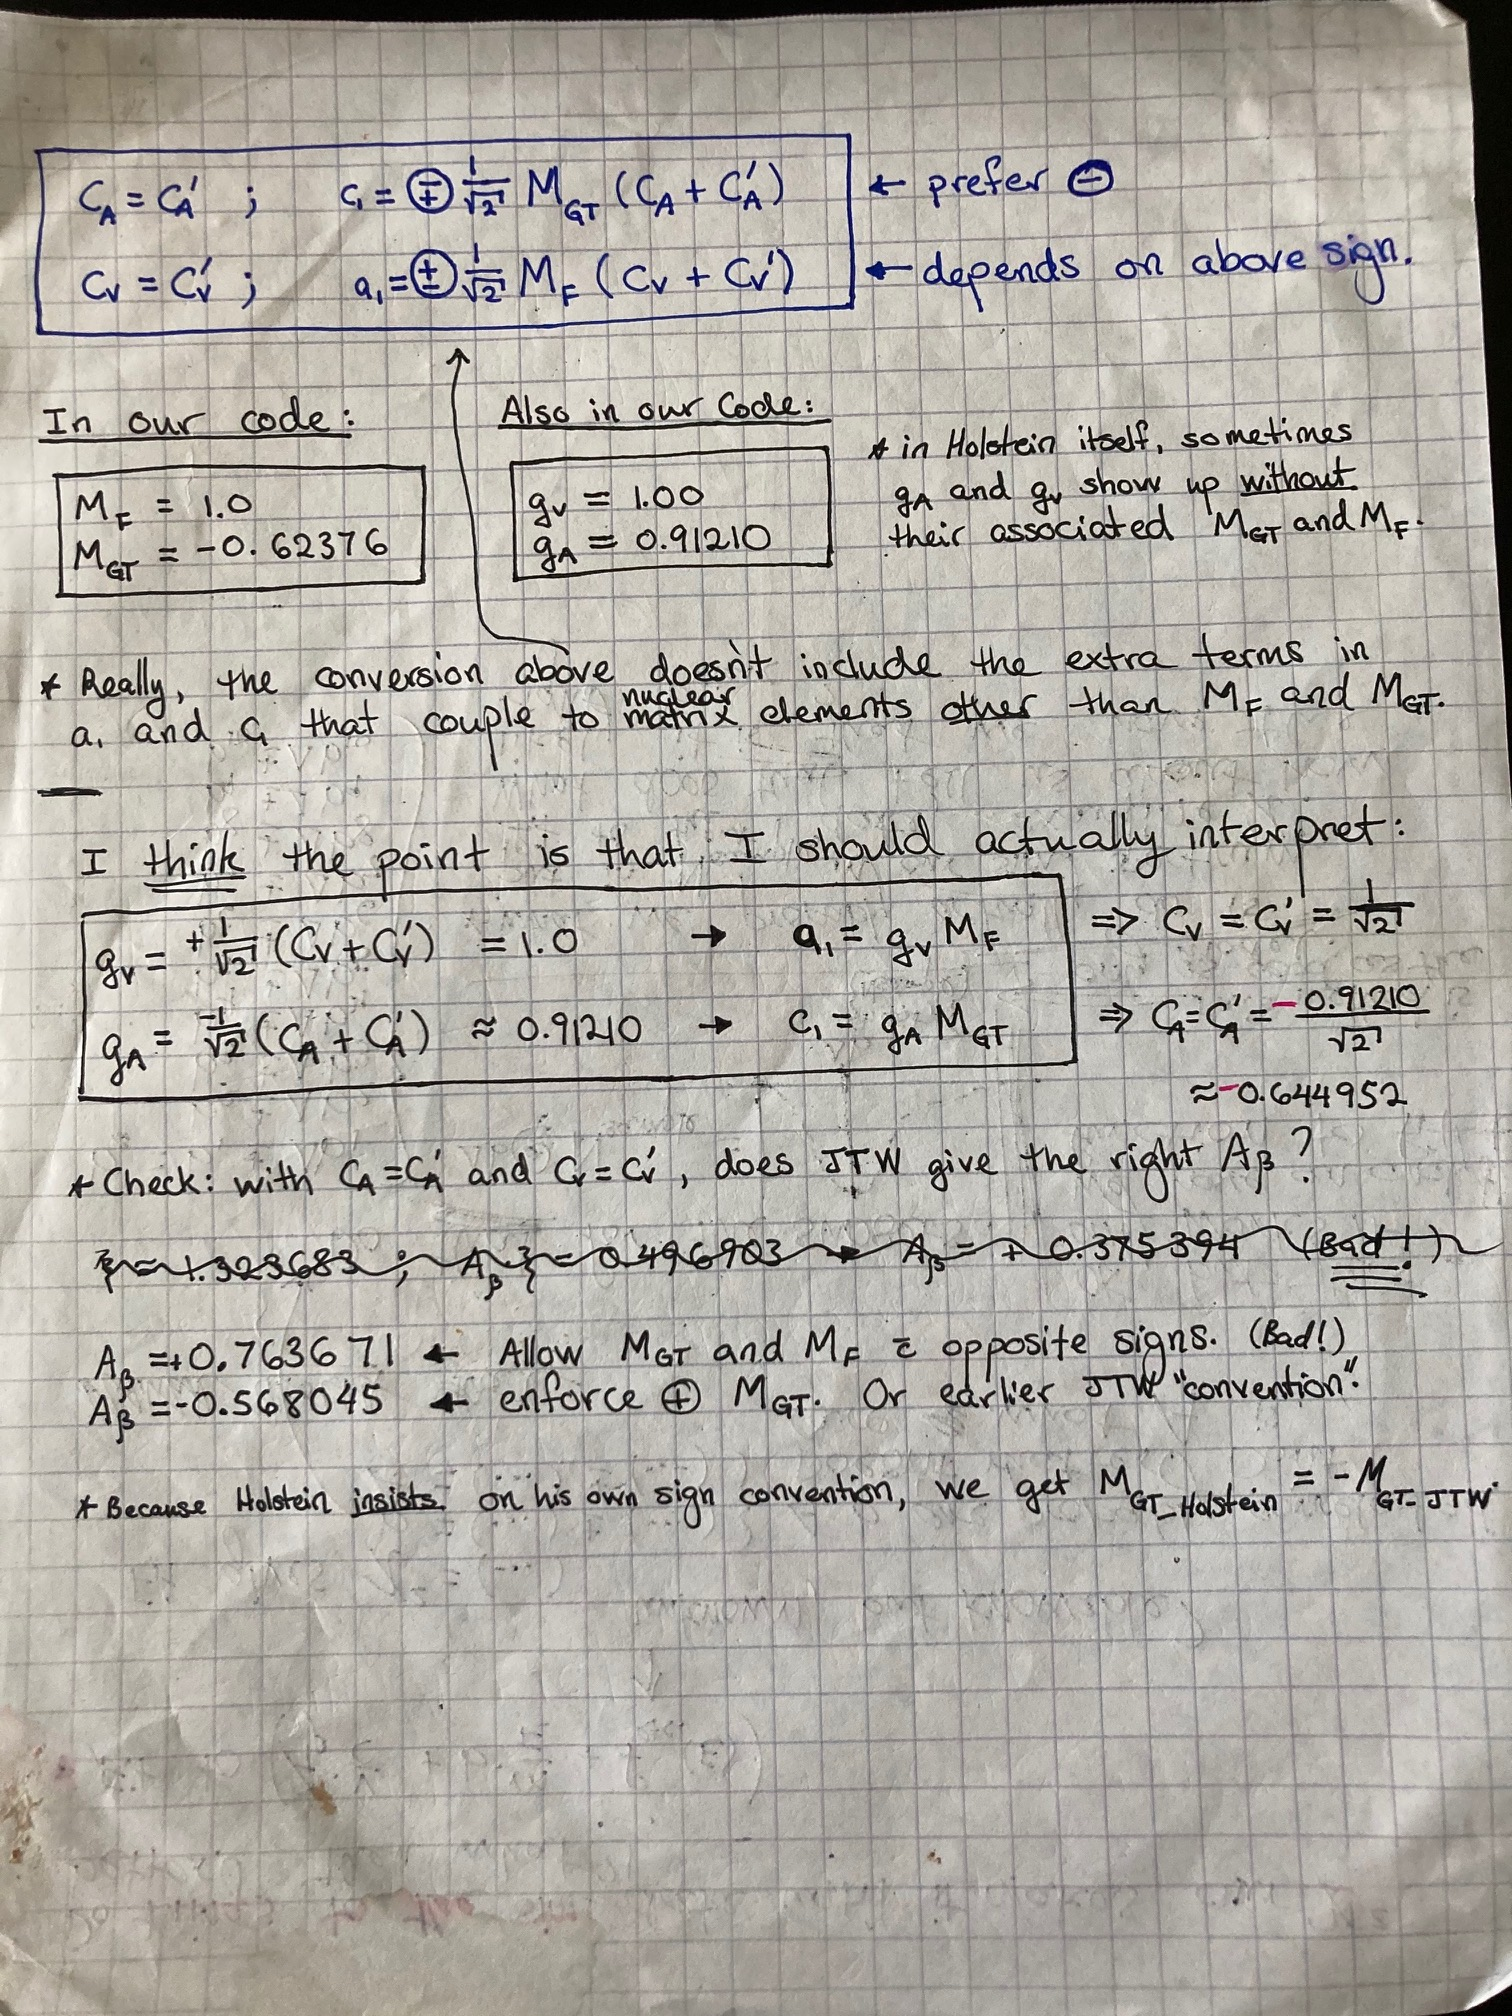
\includegraphics[width=.999\linewidth]
	{Figures/oldnotes_holstein_jtw/image0.jpg} }
	\caption{"Notes 0"}
	\label{fig:notes0}
\end{figure}

\begin{figure}[htb]
	\centering
	{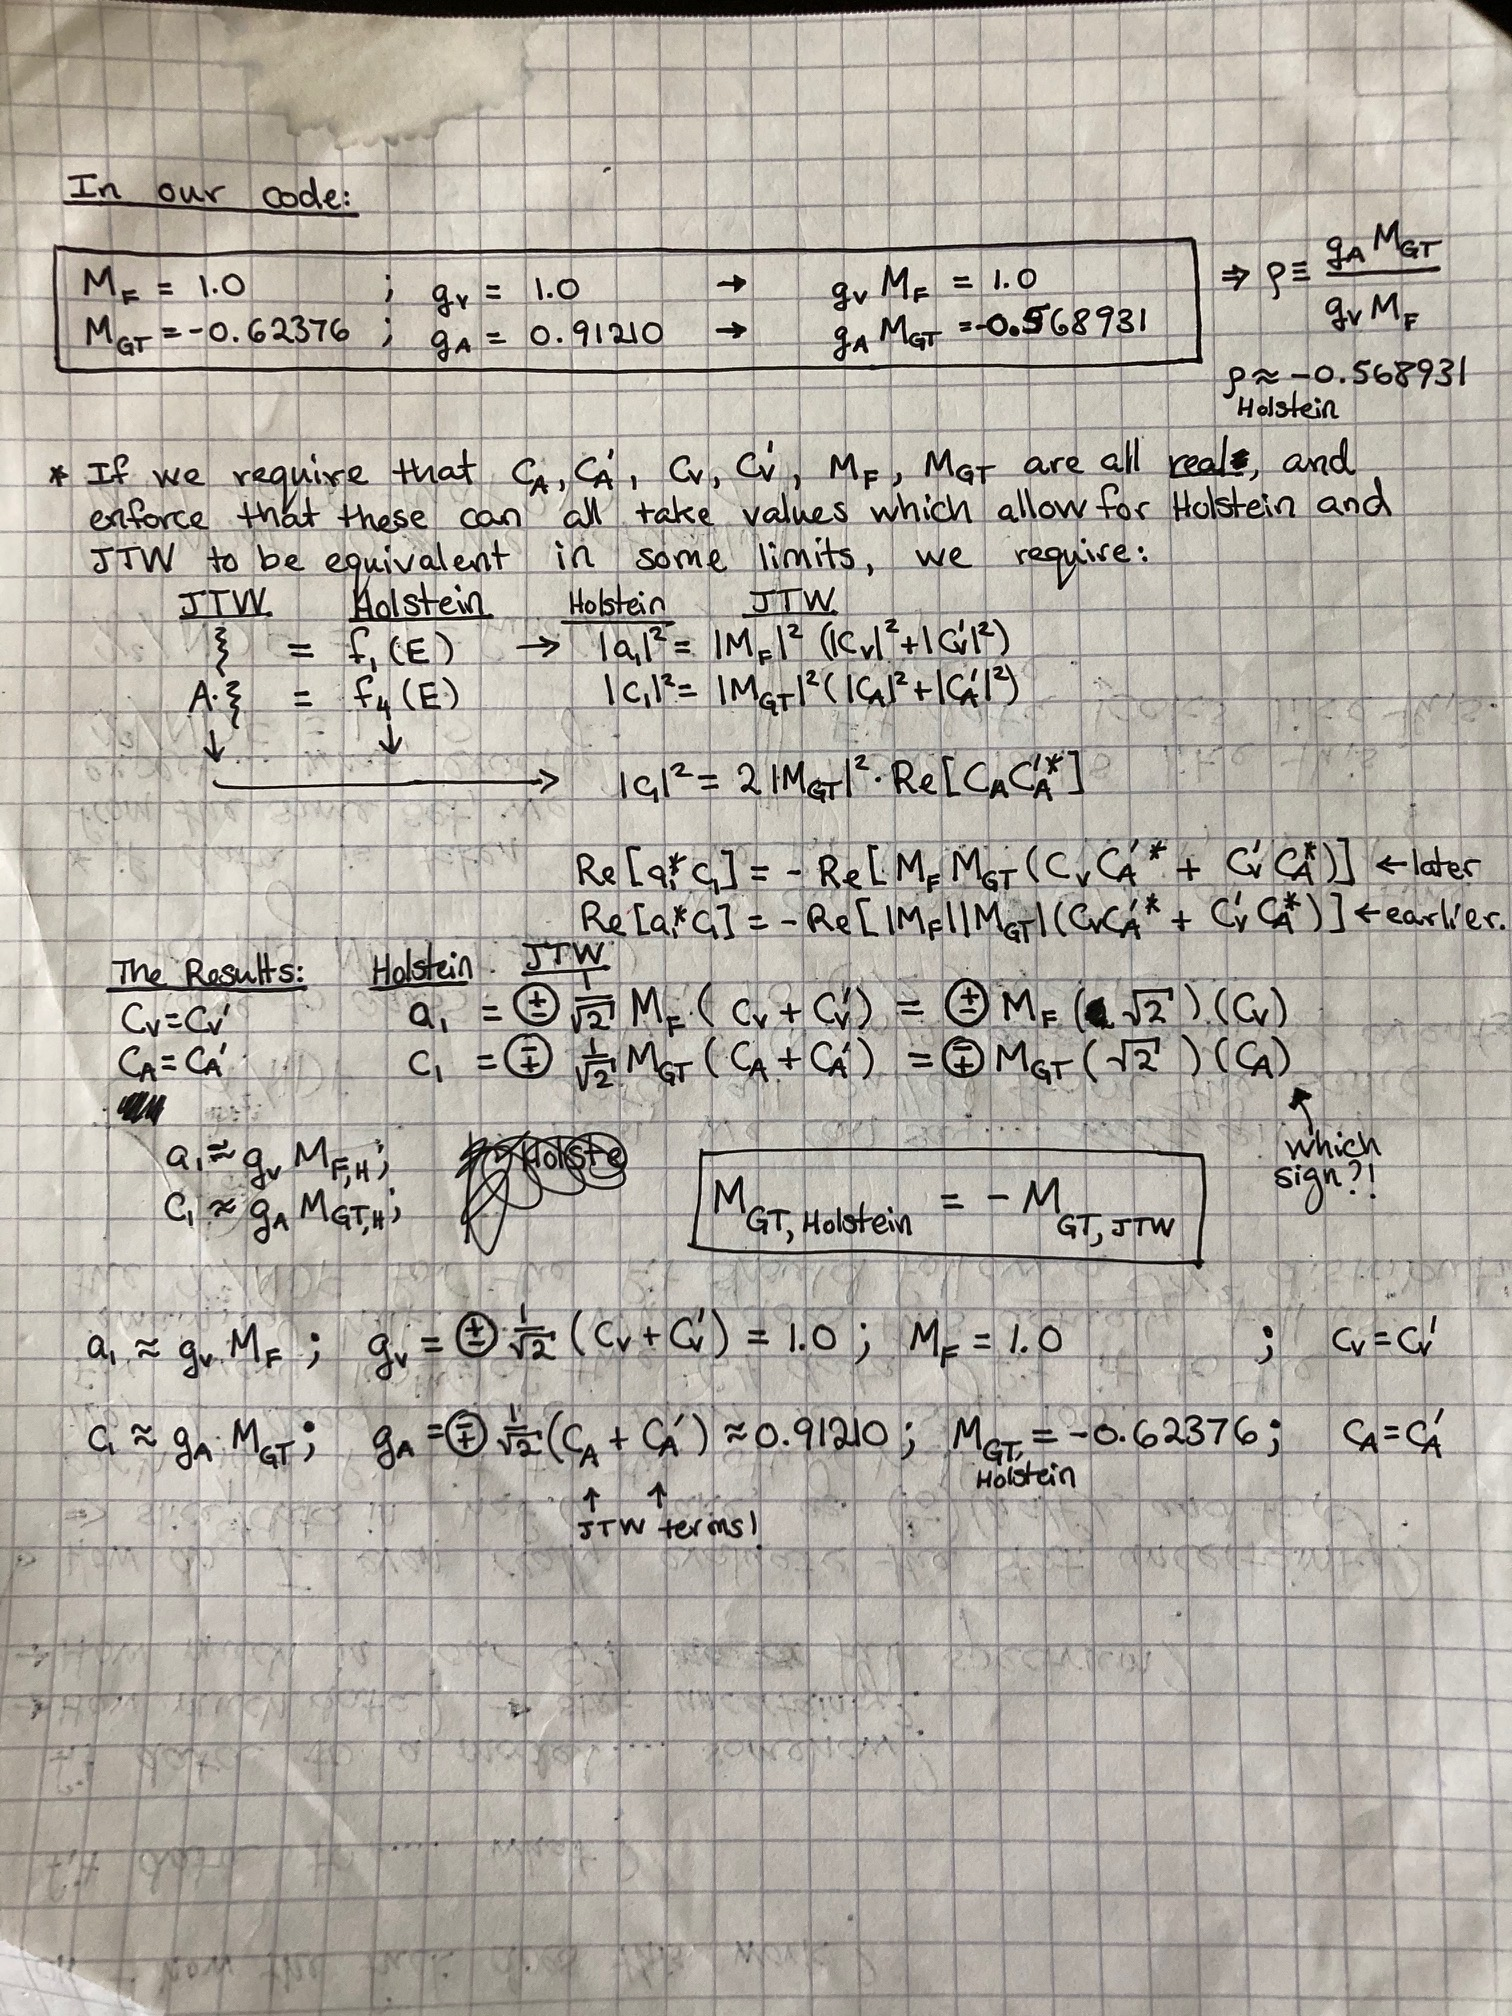
\includegraphics[width=.999\linewidth]
	{Figures/oldnotes_holstein_jtw/image1.jpg} }
	\caption{"Notes 1"}
	\label{fig:notes1}
\end{figure}

\begin{figure}[htb]
	\centering
	{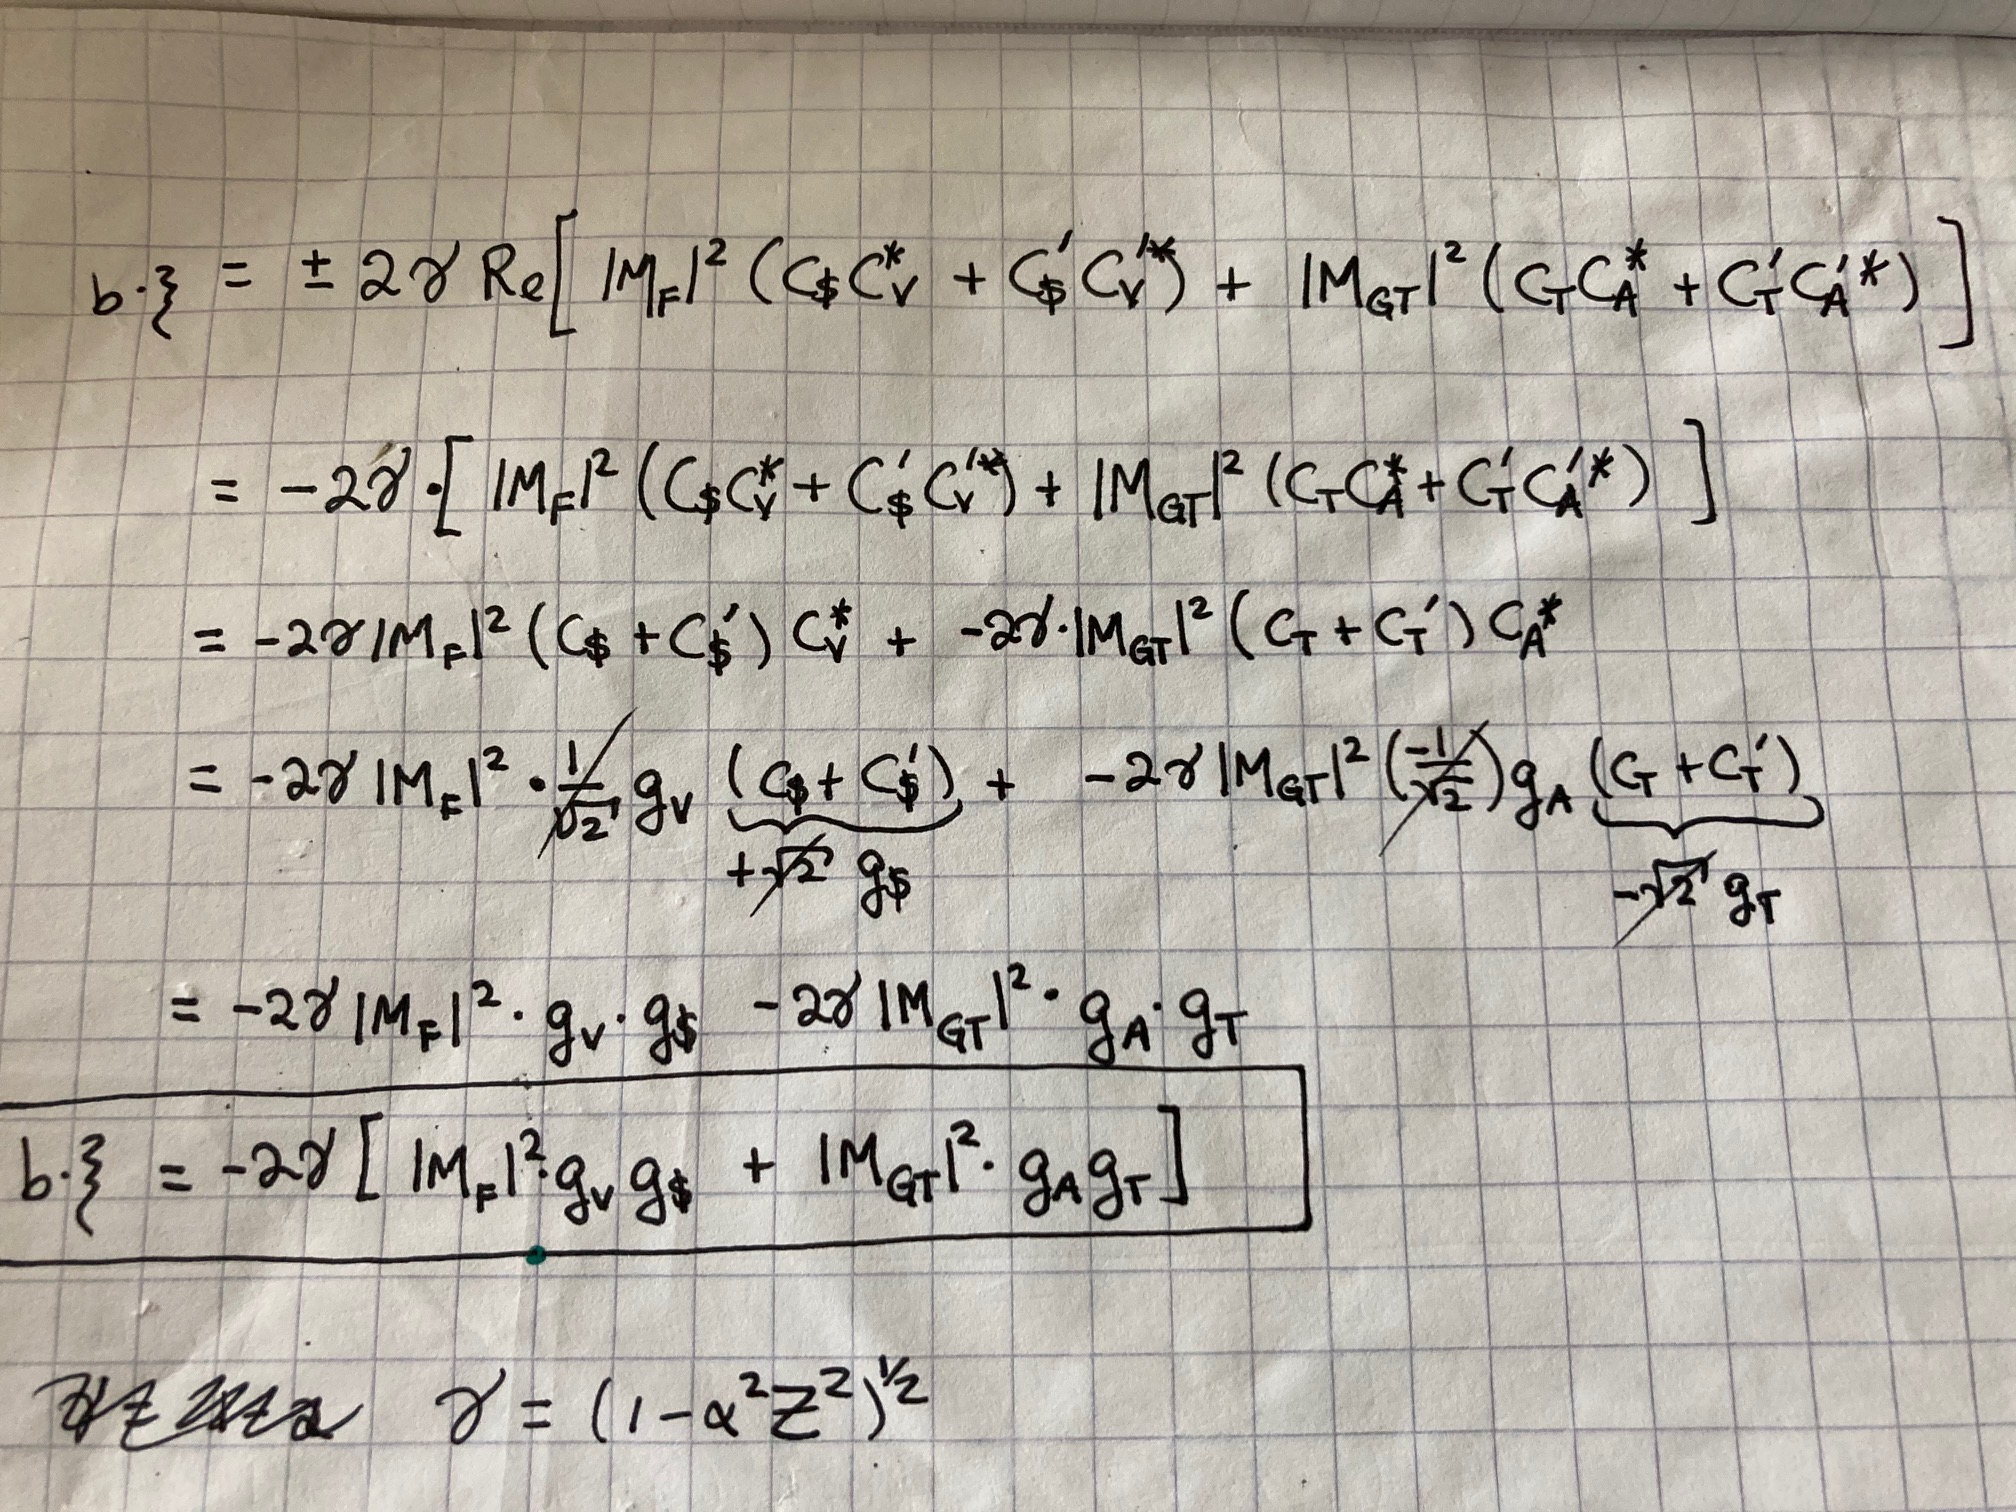
\includegraphics[width=.999\linewidth]
	{Figures/oldnotes_holstein_jtw/image2.jpg} }
	\caption{"Notes 2"}
	\label{fig:notes2}
\end{figure}

\begin{figure}[htb]
	\centering
	{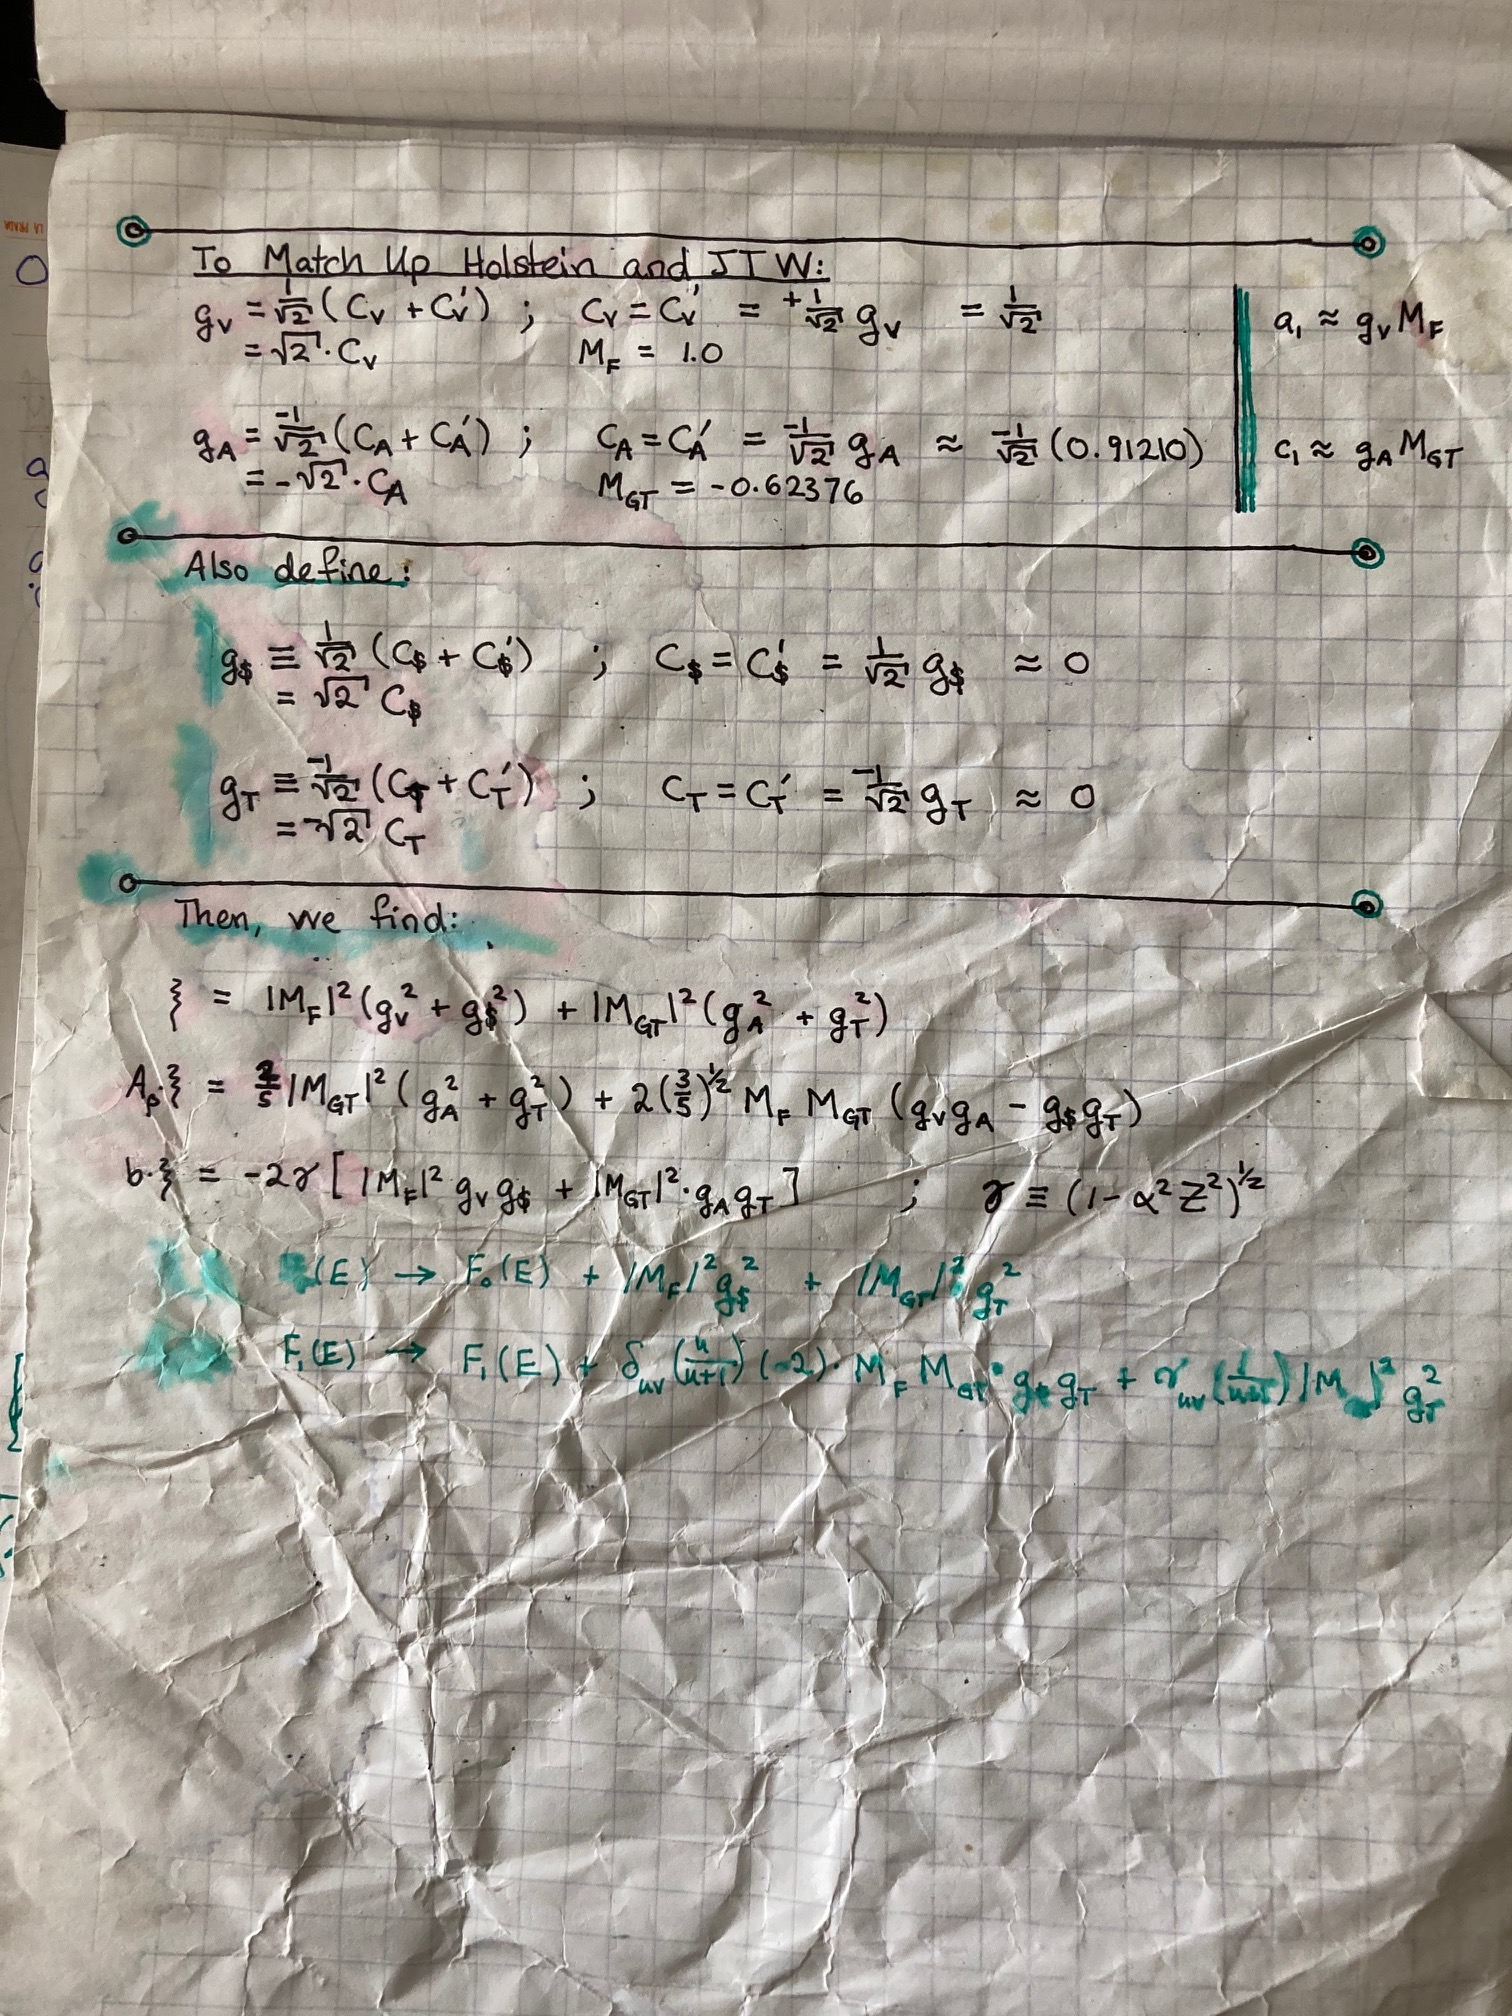
\includegraphics[width=.999\linewidth]
	{Figures/oldnotes_holstein_jtw/image3.jpg} }
	\caption{"Notes 3"}
	\label{fig:notes3}
\end{figure}

\begin{figure}[htb]
	\centering
	{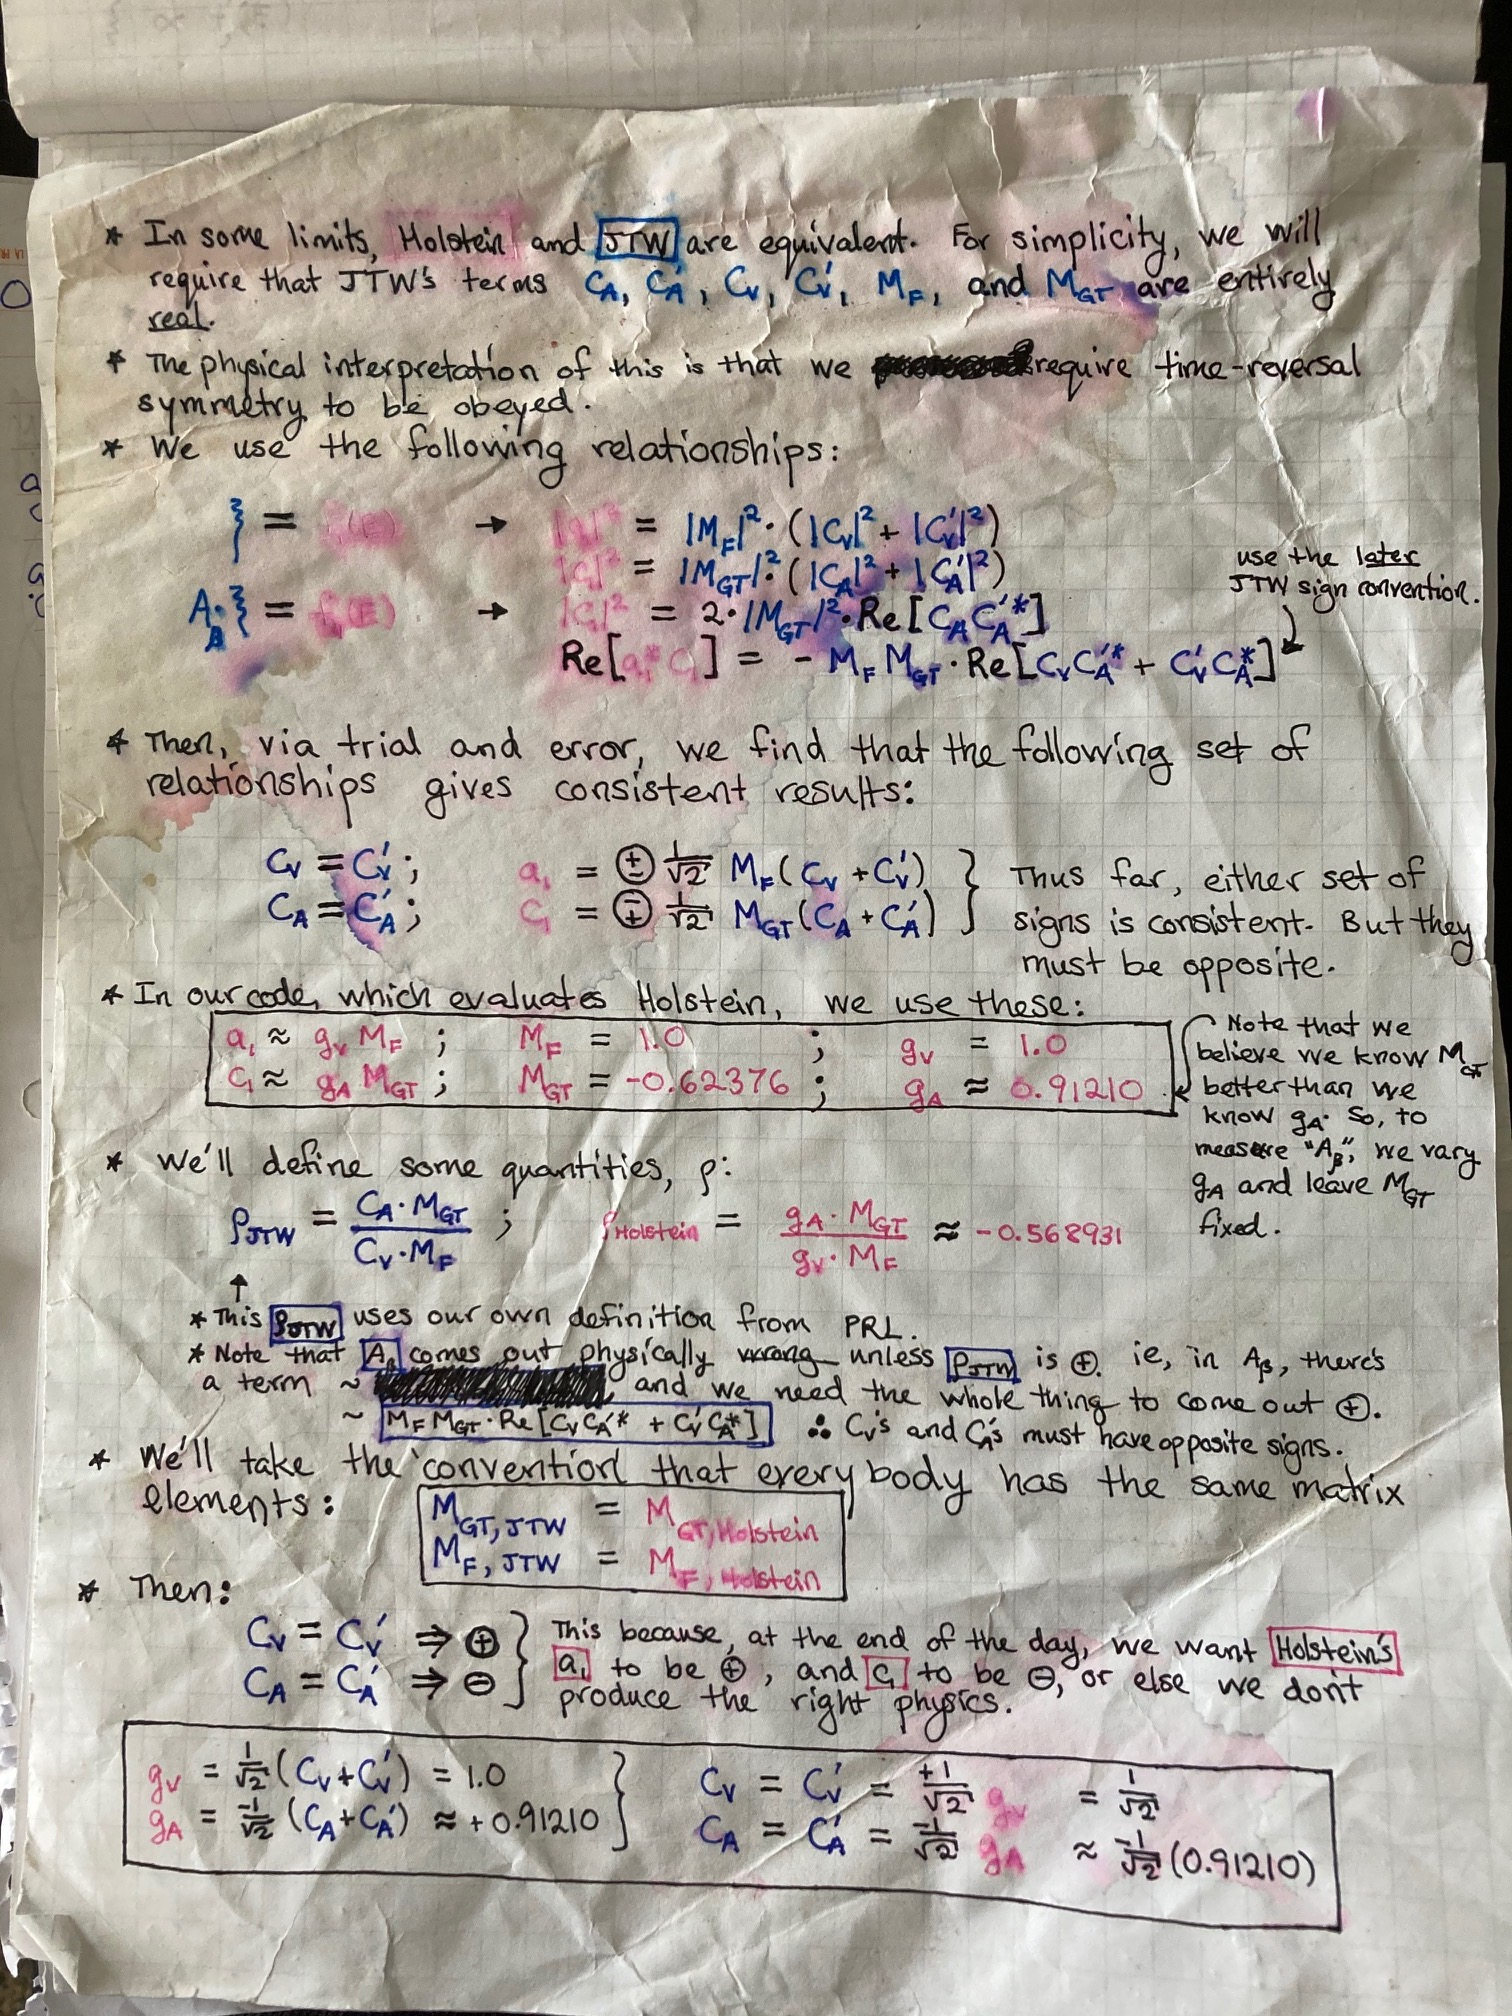
\includegraphics[width=.999\linewidth]
	{Figures/oldnotes_holstein_jtw/image4.jpg} }
	\caption{"Notes 4"}
	\label{fig:notes4}
\end{figure}

\begin{figure}[htb]
	\centering
	{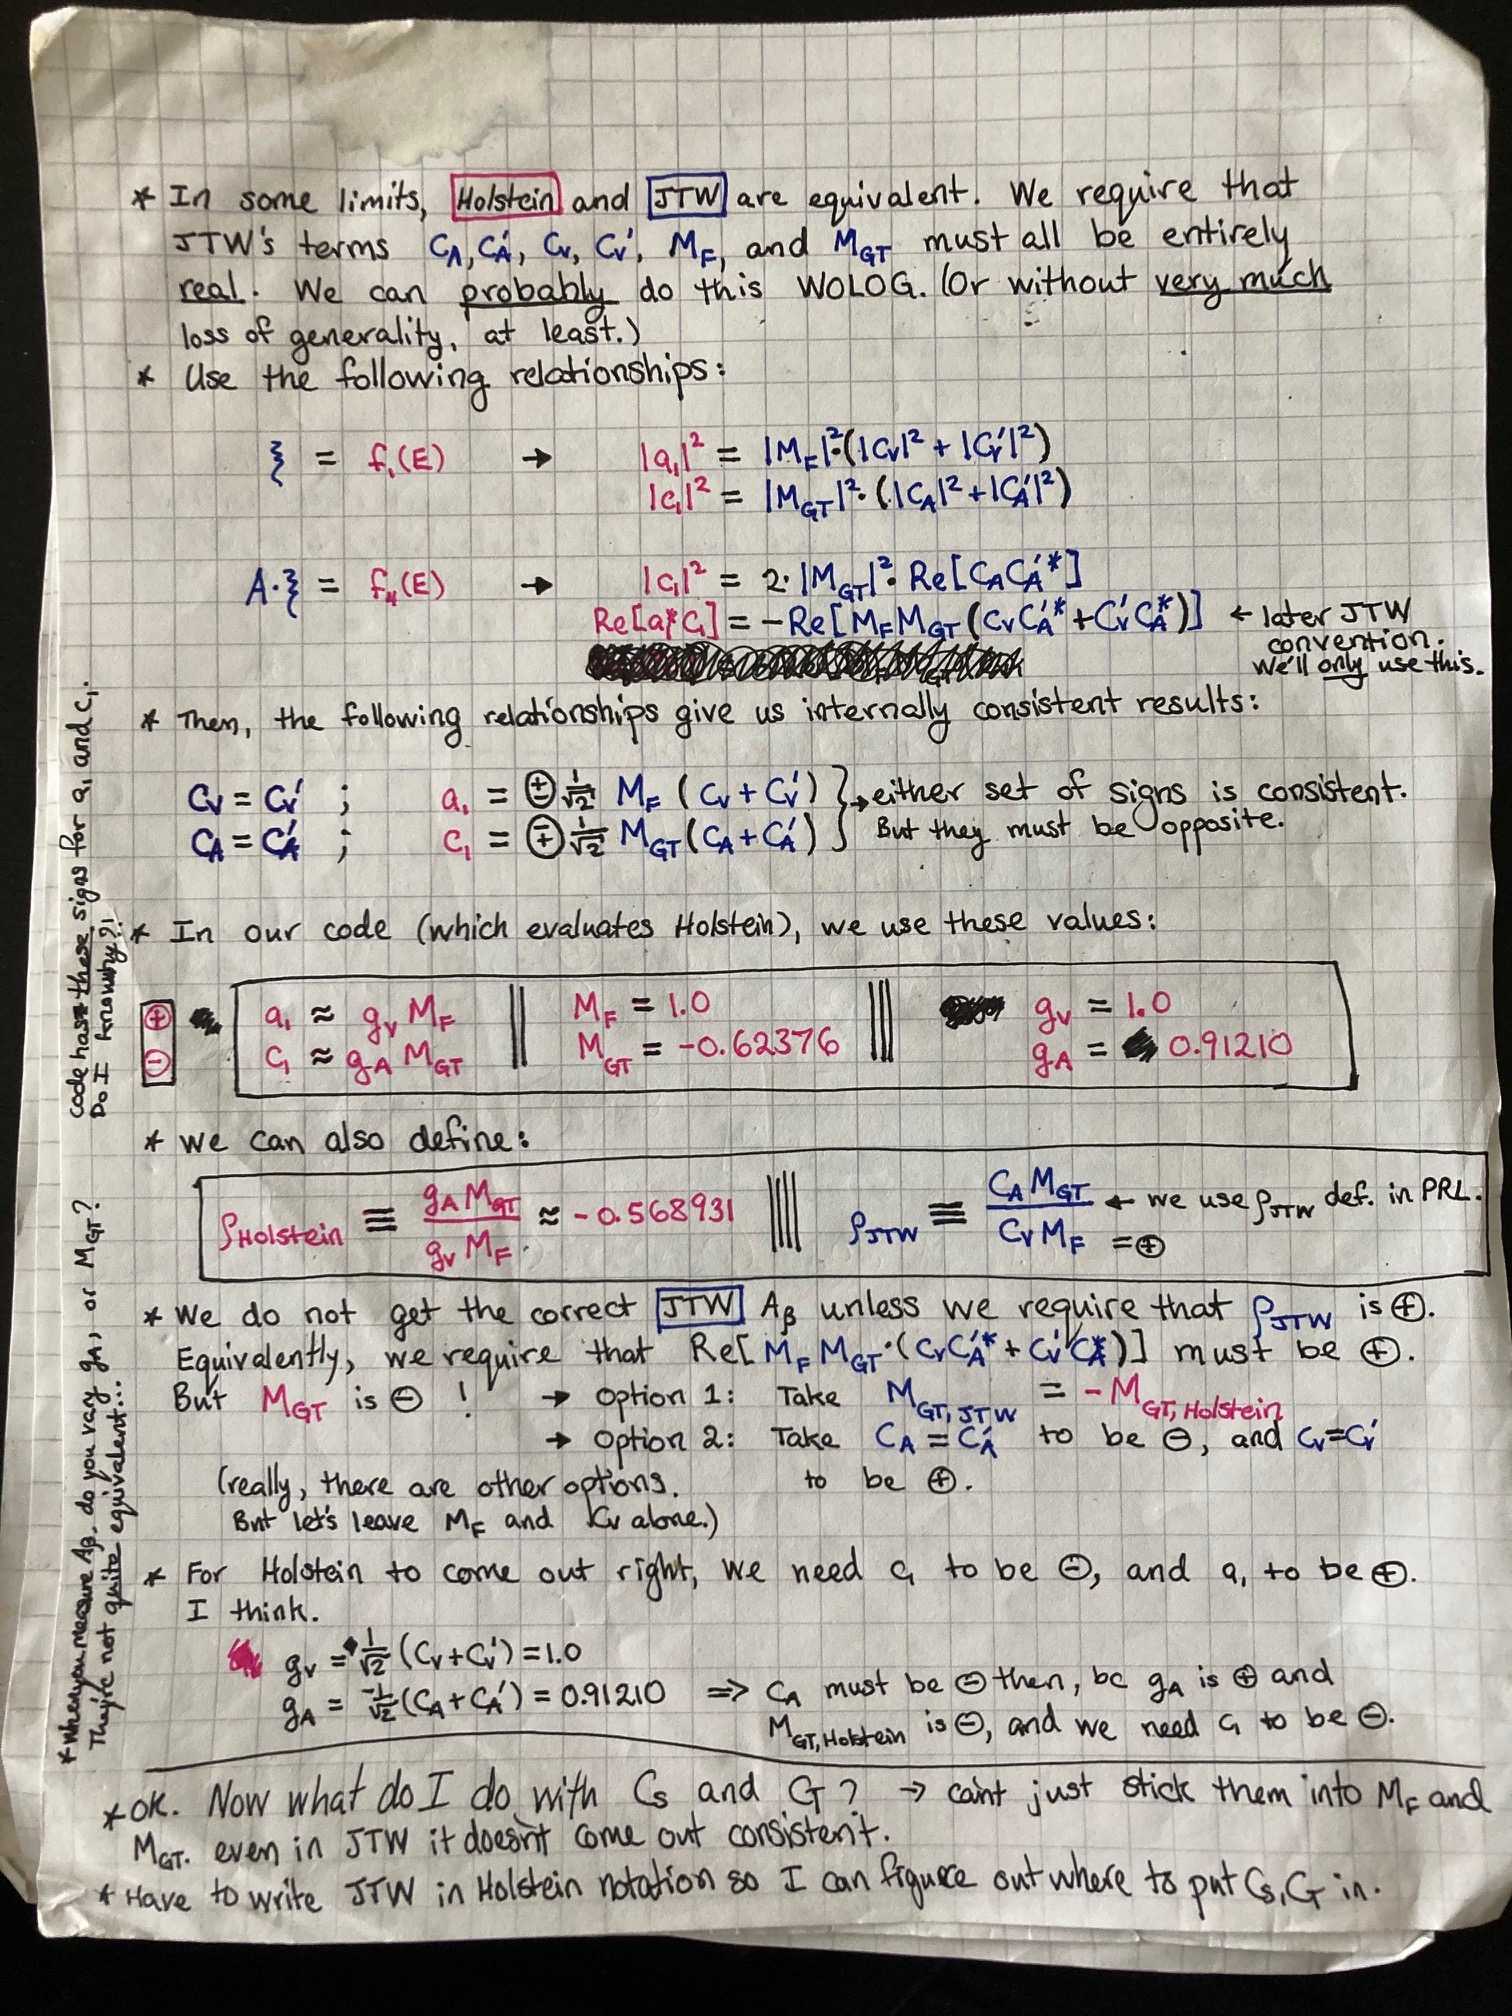
\includegraphics[width=.999\linewidth]
	{Figures/oldnotes_holstein_jtw/image5.jpg} }
	\caption{"Notes 5"}
	\label{fig:notes5}
\end{figure}


